\section{Taylorrreihen}
\begin{definition}{Definition Potenzreihen}\\
  \begin{itemize}
    \item Eine Potenzreihe ist eine undendliche Reihe vom Typ:
  \[p(x)=a_0+a_1x+a_2x^2+ \ldots = \sum_{k=0}^{\infty}{a_kx^k} \]
Die reellen Zahlen \(a_0,a_1, \ldots\) sind die Koeffizientend der Potenzreihe
  \item Allgemein können Potenzreihen mit einer verschiebung von \(x_0\) beschrieben werden, somit ist es eine
    Potenzreihe mit Zentrum \(x_0\):
    \[p(x)=a_0+a_1(x-x_0)+a_2(x-x_0)^2+\ldots = \sum_{k=0}^{\infty}{a_k(x-x_0)^k}\]
\end{itemize}
\end{definition}
\begin{definition}{Definition Taylorreihe}\\
  \begin{itemize}
    \item Die Taylorreihe oder Taylorentwicklung einer Funktion \(y=f(x)\) and der Stelle \(x_0\) ist die Potenzreihe:
      \[t_f(x)=\sum_{k=0}^{\infty}{a_k(x-x_0)^k}\]
      welche die gleiche Ableitung an der Stelle \(x_0 \text{ für alle }k\in \mathbb{N}\) hat wie die Funktion \(f(x)\)
  \end{itemize}
\end{definition}
\begin{definition}{Definition Taylorpolynom}\\
    \begin{itemize}
      \item Ein Taylorpolynom ist eine Taylorreihe \(t_f(x)\) welche nach \(n\text{-ter}\) Ordnung abgebrochen wird.
        Somit erhällt man das Taylorpolynom \(n\text{-ter}\) Ordnung von \(f(x)\) an der Stelle \(x_0\):
        \[p_n(x)=\sum_{k=0}^n{a_k(x-x_0)^k}\]
    \end{itemize}
  \begin{centering}
  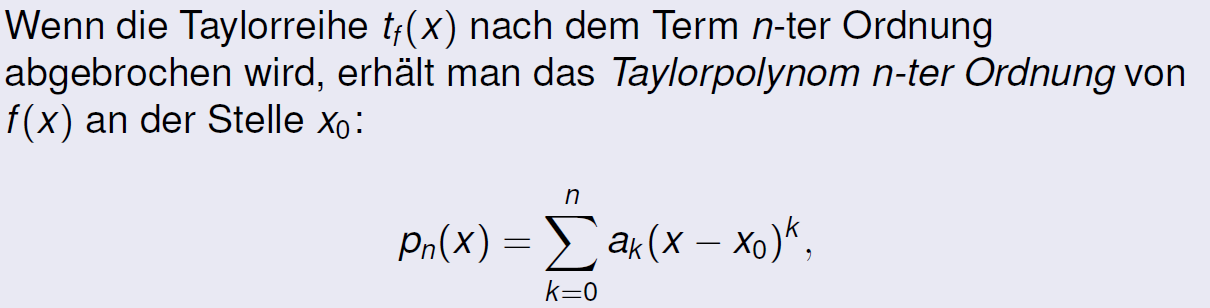
\includegraphics[width=0.8\textwidth]{images/2024-06-02-19-16-13.png}\\
  \end{centering}
  \begin{centering}
  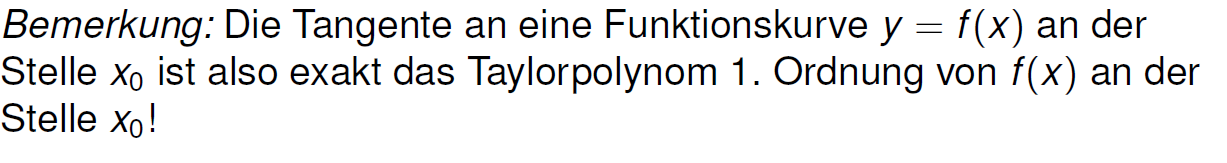
\includegraphics[width=0.8\textwidth]{images/2024-06-02-19-16-27.png}\\
  \end{centering}
\end{definition}
\begin{KR}{Vorgehen Berechnen Taylorreihe}\\
  \begin{centering}
  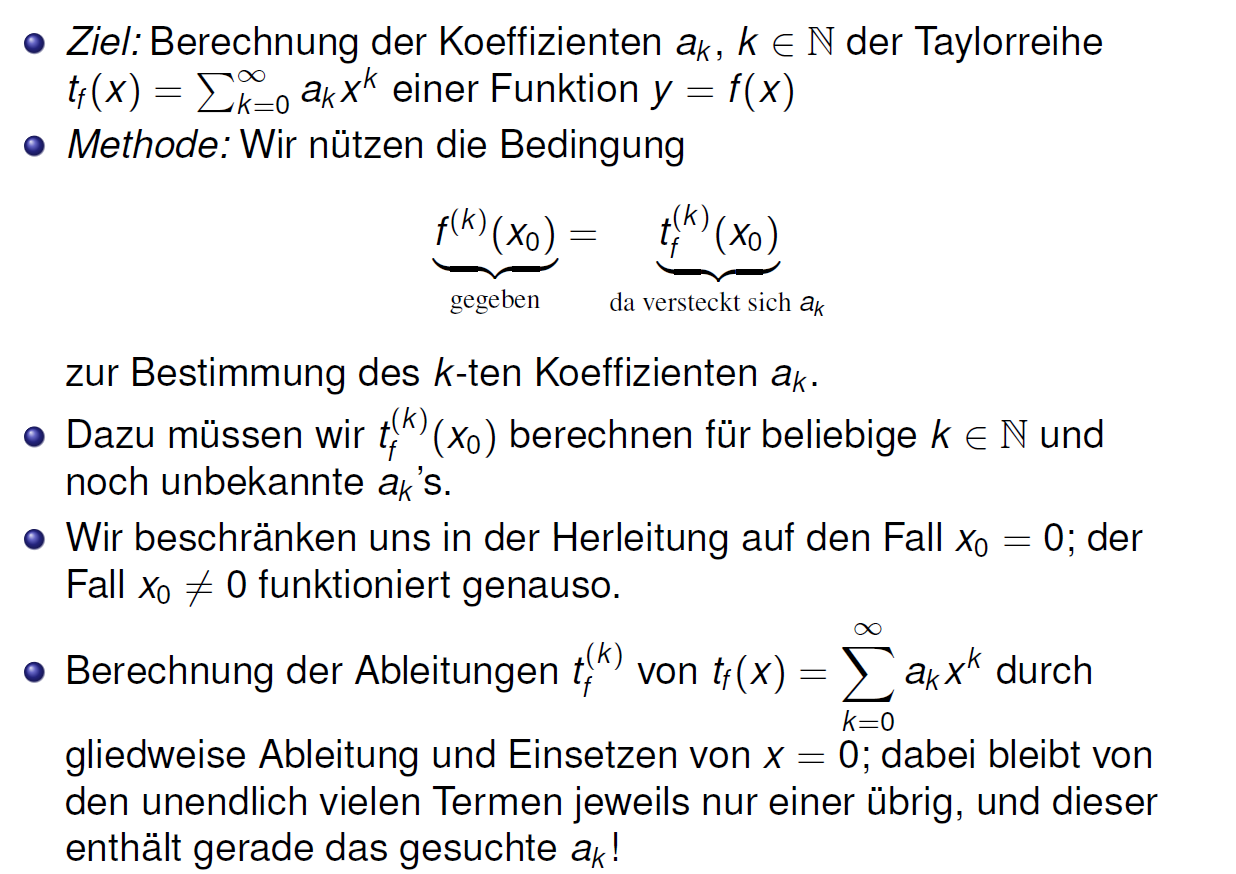
\includegraphics[width=0.8\textwidth]{images/2024-06-02-19-18-15.png}\\
  \end{centering}
\end{KR}
\begin{formula}{Formel für Taylorkoeffizienten}\\
  \begin{centering}
  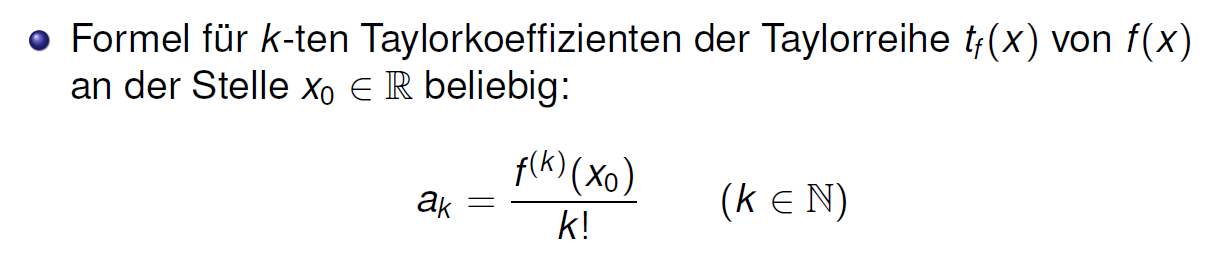
\includegraphics[width=0.8\textwidth]{images/2024-06-02-19-21-01.png}\\
  \end{centering}
  \begin{centering}
  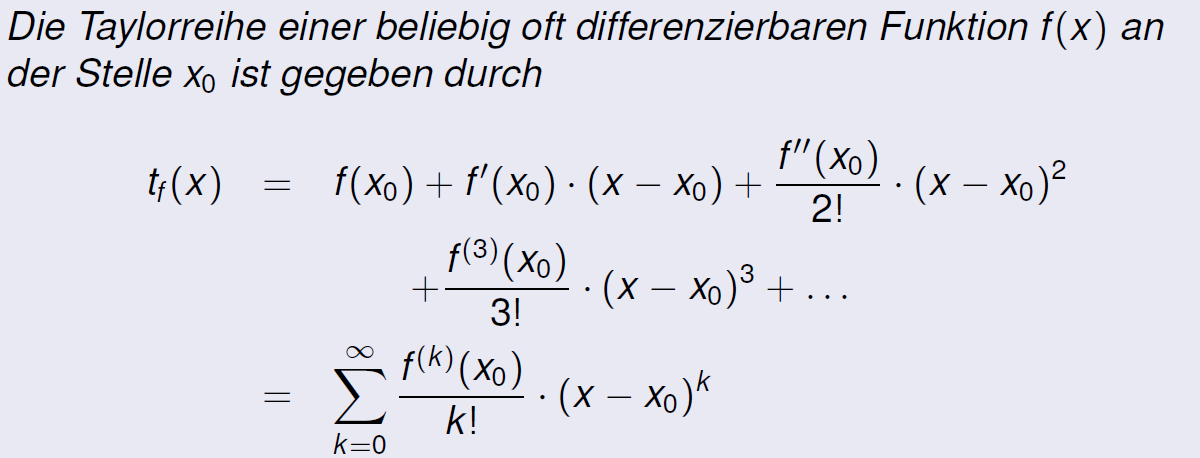
\includegraphics[width=0.8\textwidth]{images/2024-06-02-19-24-01.png}\\
  \end{centering}
\end{formula}
\subsection{Symetrie von Potenzreihen und Taylorreihen}
\begin{lemma}{Symetrie von Funktionen}\\
  \begin{centering}
    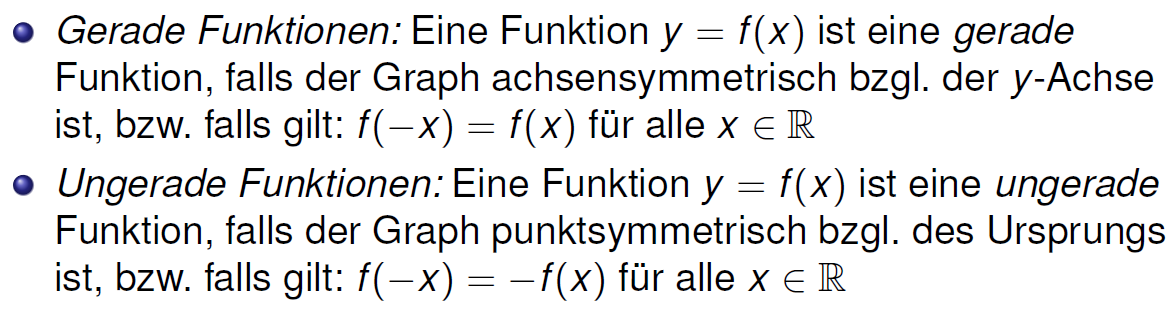
\includegraphics[width=0.8\textwidth]{images/2024-06-02-19-25-55.png}\\
  \end{centering} 
\end{lemma}
\begin{lemma}{Symetrie von Potenzreihen}\\
  \begin{centering}
  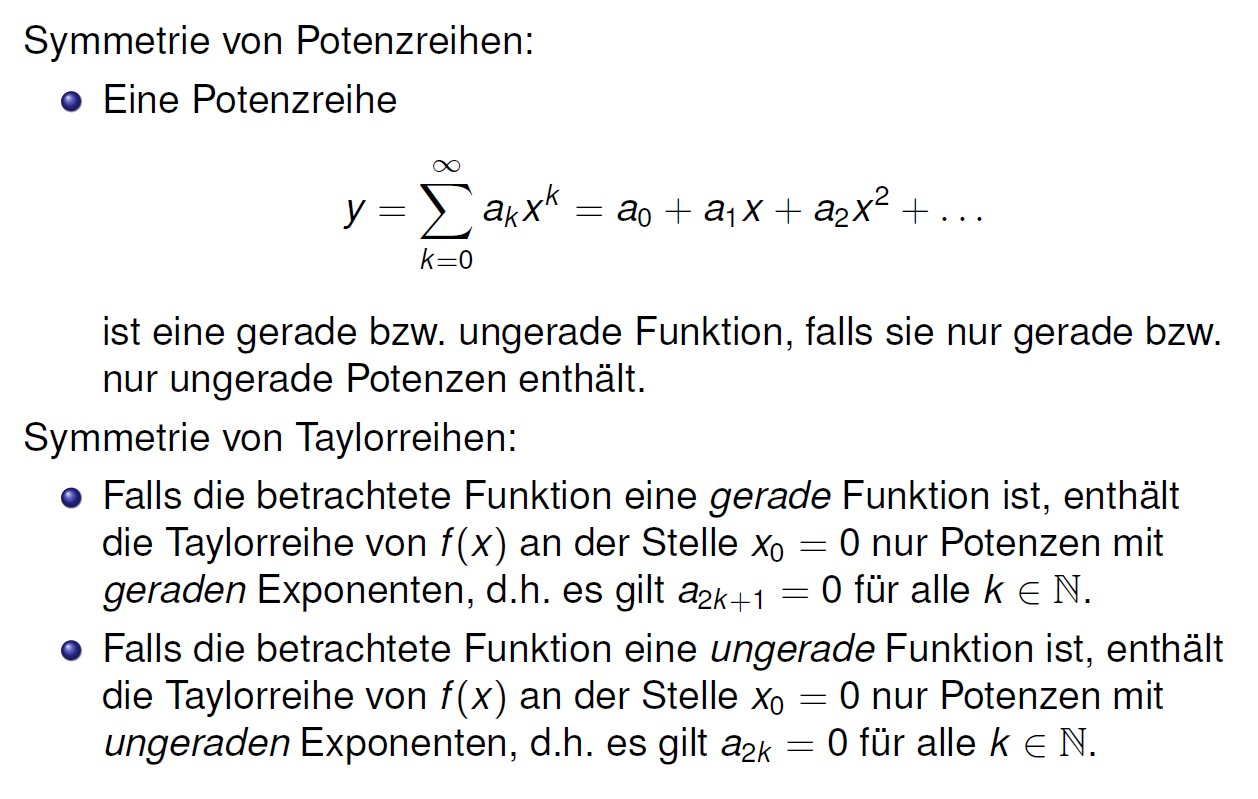
\includegraphics[width=0.8\textwidth]{images/2024-06-02-19-28-18.png}\\
  \end{centering}
\end{lemma}
\begin{lemma}{Binomialkoeffizienten}\\
  \begin{centering}
  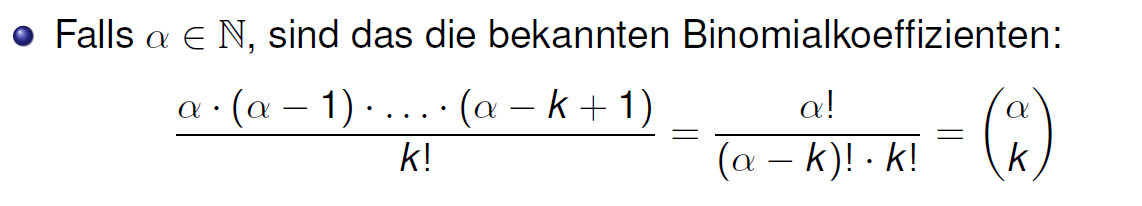
\includegraphics[width=0.8\textwidth]{images/2024-06-02-19-31-35.png}\\
  \end{centering}
  \begin{centering}
  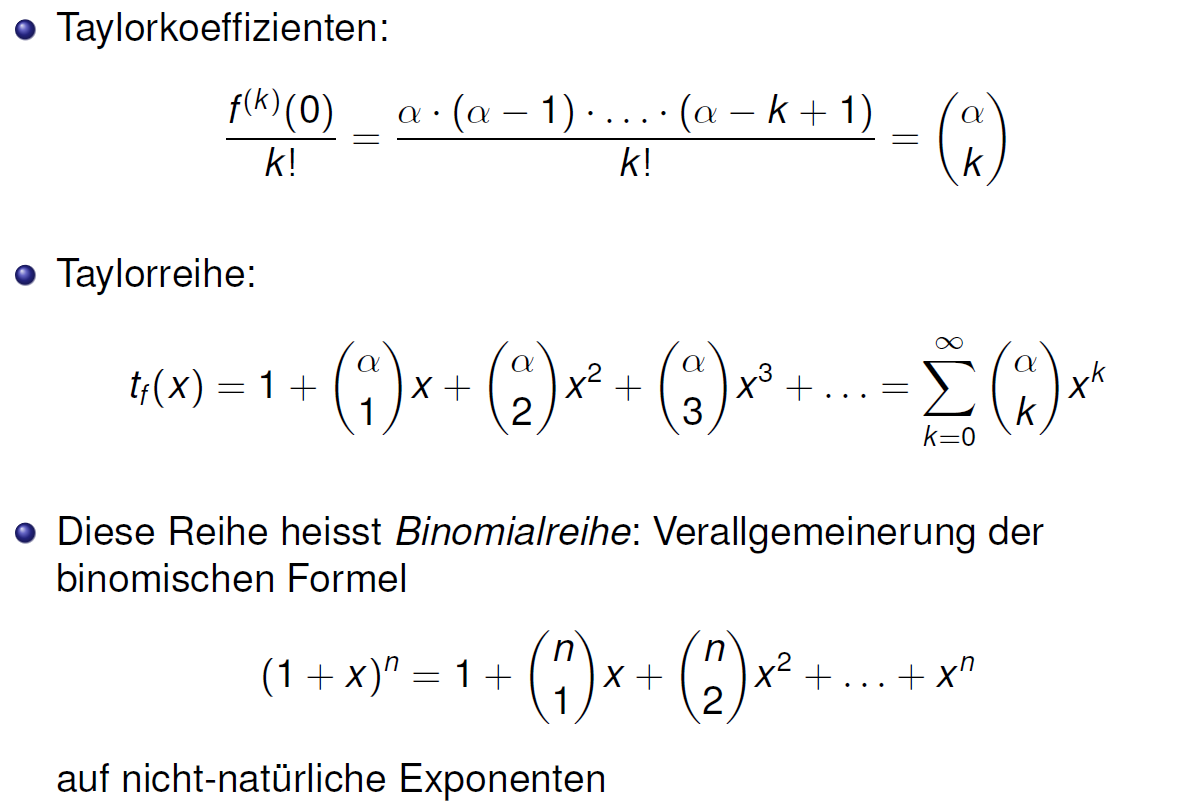
\includegraphics[width=0.8\textwidth]{images/2024-06-02-19-32-15.png}\\
  \end{centering}
\end{lemma}
\begin{definition}{Regel von Bernoulli- de l’Hospital}\\
  \begin{centering}
  
\includegraphics[width=0.8\textwidth]{images/2024-06-02-21-42-08.png}\\
  \end{centering}
  \begin{centering}
  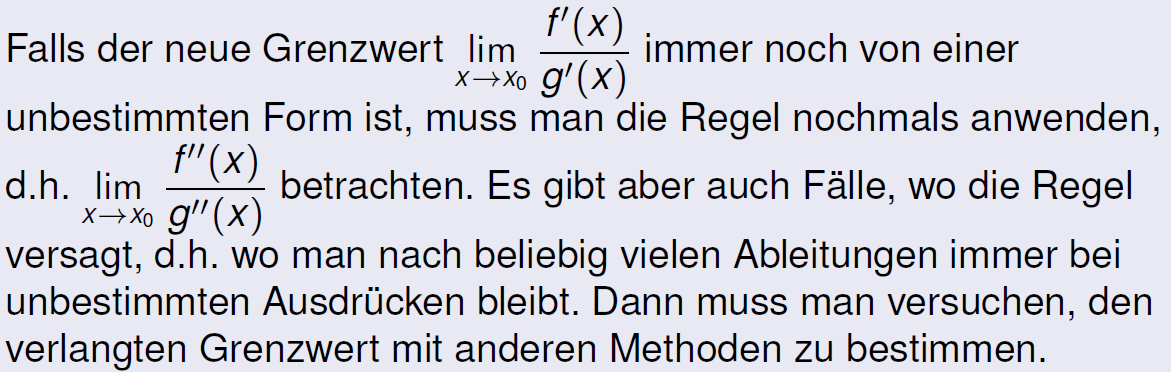
\includegraphics[width=0.8\textwidth]{images/2024-06-02-21-42-41.png}\\
  \end{centering}
\end{definition}
\begin{definition}{Varianten von l'Hospital}\\
  \begin{centering}
  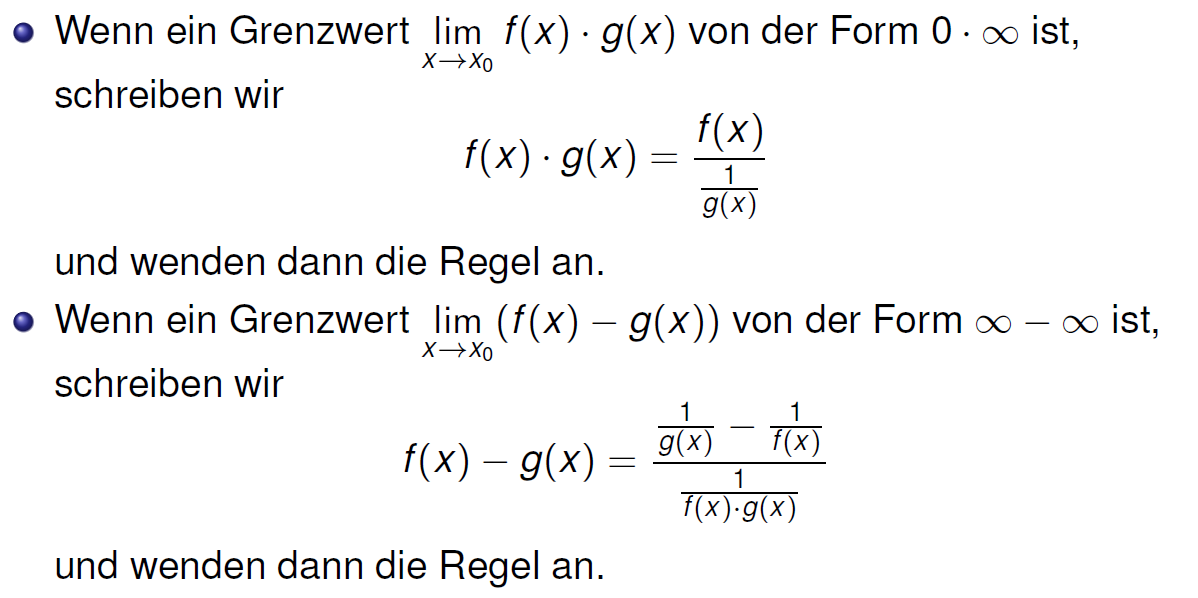
\includegraphics[width=0.8\textwidth]{images/2024-06-02-21-43-36.png}\\
  \end{centering}
\end{definition}
\begin{definition}{Genauigkeit der Approximation}\\
  \begin{centering}
  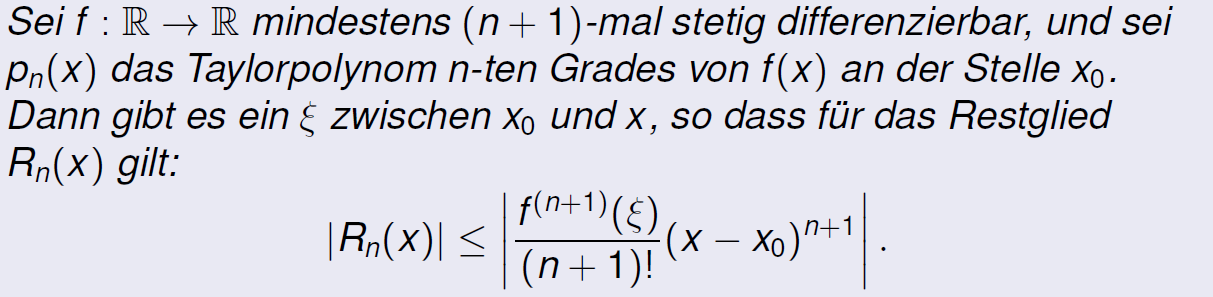
\includegraphics[width=0.8\textwidth]{images/2024-06-02-21-45-47.png}\\
  \end{centering}
\end{definition}
\subsection{Konvergenz von Potenzreihen}
\begin{definition}{Konvergenzradius}\\
  \begin{centering}
  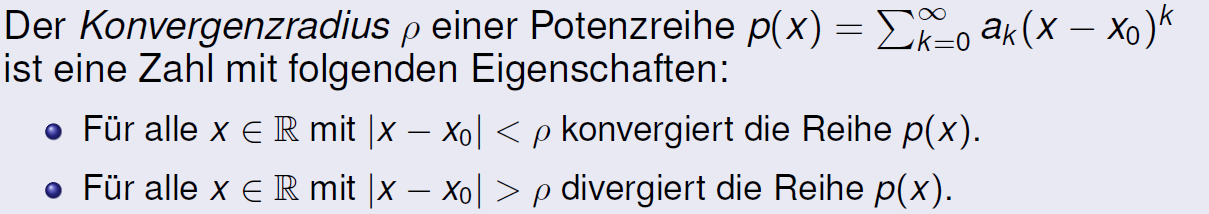
\includegraphics[width=0.8\textwidth]{images/2024-06-02-21-48-37.png}\\
  \end{centering}
  \begin{centering}
  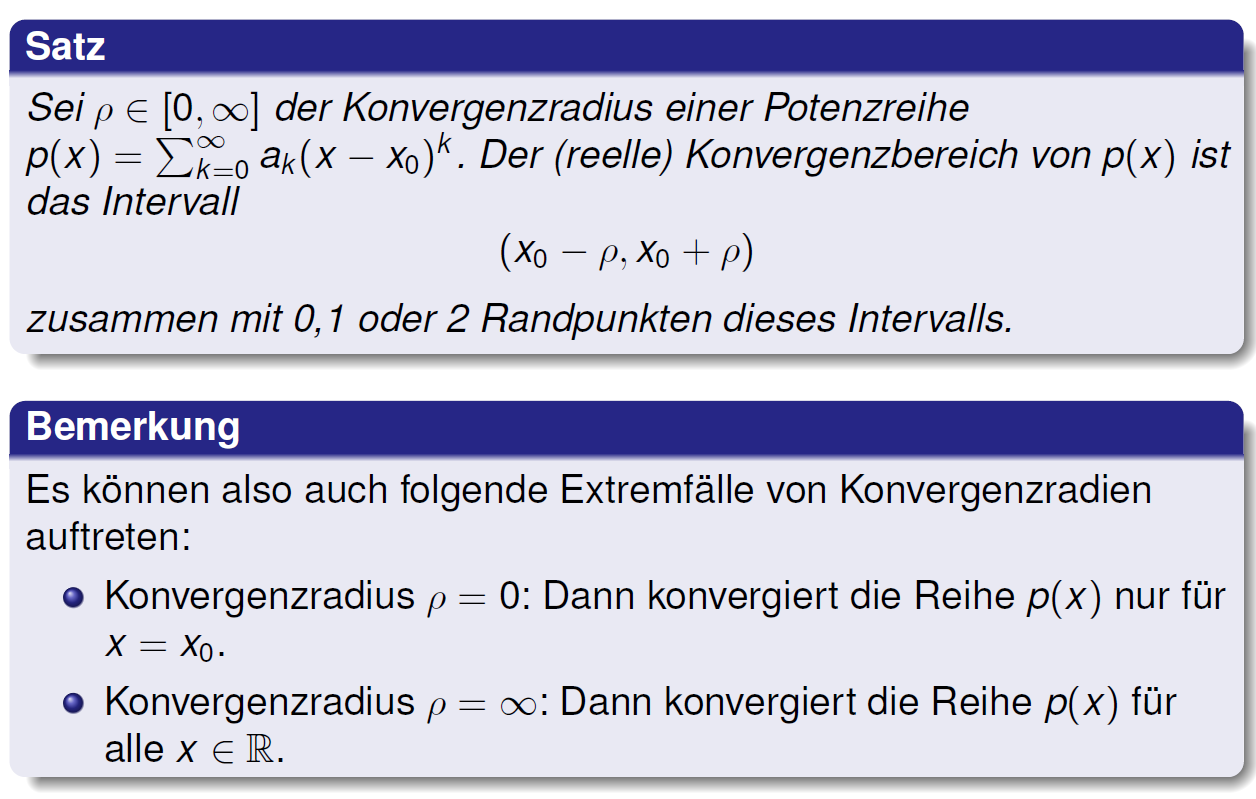
\includegraphics[width=0.8\textwidth]{images/2024-06-02-21-53-30.png}\\
  \end{centering}
\end{definition}
\begin{formula}{Konvergenzradius Formel}
  \begin{centering}
  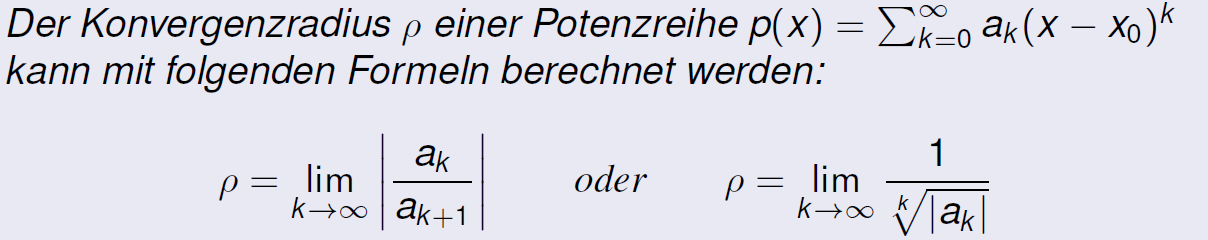
\includegraphics[width=0.8\textwidth]{images/2024-06-02-21-54-17.png}\\
  \end{centering}
\end{formula}
